% Figures for Pi, Screen and Power Consumption
\begin{figure*}
  \begin{minipage}[t]{0.22\textwidth}
    \centering
    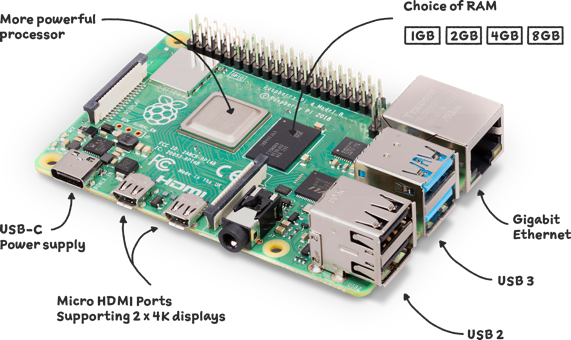
\includegraphics[width=\textwidth]{imgs/pi4_labelled.png}
    \caption{Raspberry Pi 4 Model B 2GB\cite{pi4}}
  \end{minipage}
  \hfill
  \begin{minipage}[t]{0.22\textwidth}
    \centering
    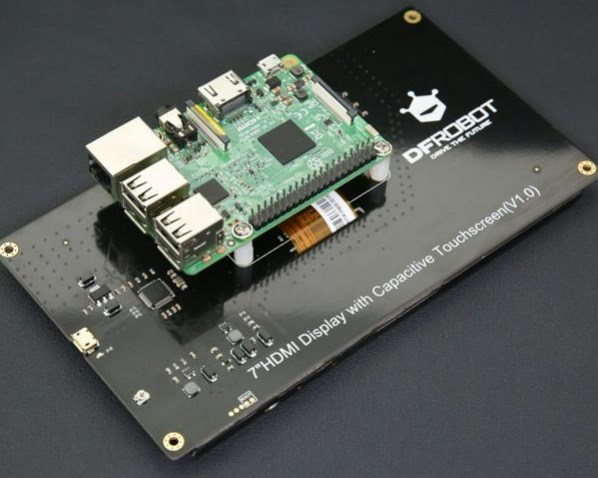
\includegraphics[width=\textwidth]{imgs/dfrobot_screen.jpg}
    \caption{DFRobot 7" Touchscreen Display\cite{7inchdisplay}}
  \end{minipage}
  \hfill
  \begin{minipage}[t]{0.22\textwidth}
      \centering
      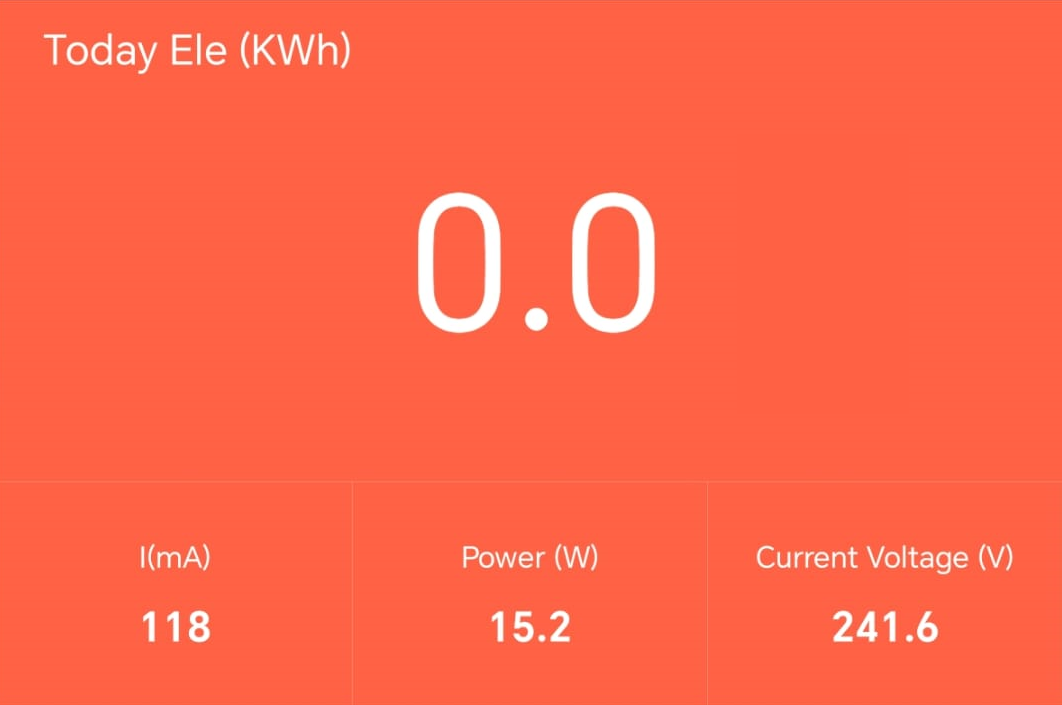
\includegraphics[width=\textwidth]{imgs/powermeter.png}
      \caption{Power consumption of the system}
  \end{minipage}
  \hfill
  \begin{minipage}[t]{0.22\textwidth}
    \centering
    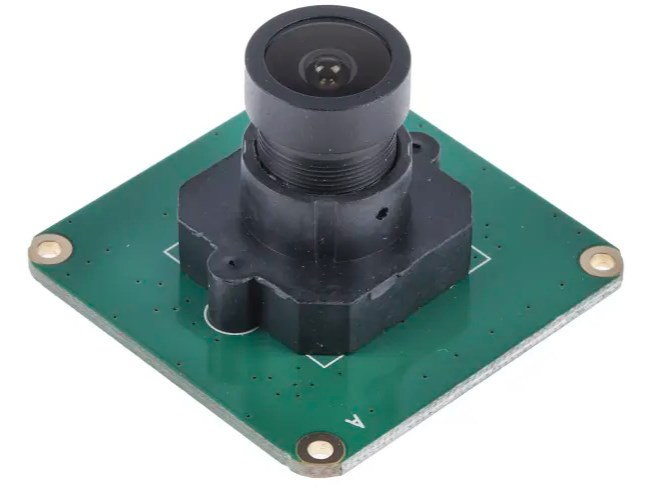
\includegraphics[width=\textwidth]{imgs/okdo_camera.jpg}
    \caption{Okdo Adjustable Focus OV5647 Camera\cite{okdocamera}}
  \end{minipage}
\end{figure*}

\subsection{Hardware, Mechanics and Electronics}
The hardware, mechanics and electronics (HME) of the system are the physical components that make up the system.
It is necassary to first consider the HME of the system as they are the foundation upon which the rest of the system is built;
for example, when designing the Computer Vision system, it should utilise training data that was collected using the HME 
that the system will be deployed on, ensuring that the system is robust to the conditions it will be used in. As such,
the main focus of this stage has been the HME.
\subsubsection{Hardware} \label{sec:hardware}
For the initial stage of the project, the main hardware components of the HME are:
\begin{mylist}
  \item Raspberry Pi 4 Model B 2GB
  \item 7" Touchscreen Display
  \item 24V dc, 6.25A, 150W Power Supply
  \item Okdo Adjustable Focus OV5647 Camera
  \item LED Light Strip
\end{mylist}
% Pi
\textbf{Raspberry Pi 4 Model B 2GB} \\
The Raspberry Pi 4 Model B is the main component of the system, and is the central hub that all other components are connected to.
This model was chosen as it is regarded as a reliable SoC and is widely used in the industry. It has a large amount of software
and driver support, so I can be confident that I will be able to find a solution to any issues that may arise. Additionally, 
it has GPIO pins that can be used to control other components which will be necassary in future stages. It also has a 
dedicated camera port which allows for a camera to be connected directly to the SoC, which is necassary for the Computer Vision system.

It also has WiFi support for SSH and remote development, as well as HDMI port for the display.
Originally, the 4GB model was ordered however an issue with the EE Stores resulted in receiving the 2GB model instead.
This was not an issue as the 2GB model is sufficient for the initial stage of the project, however if it is found to be a bottleneck
in future stages, a more powerful model may be used. The decision to not return the 2GB model is because the EEStores are not
available over the Christmas break.

% Figures for 3D Printed Frame
\subsubsection{Mechanics} \label{sec:mechanics}
\begin{figure*}
    \begin{minipage}[t]{0.32\textwidth}
      \centering
      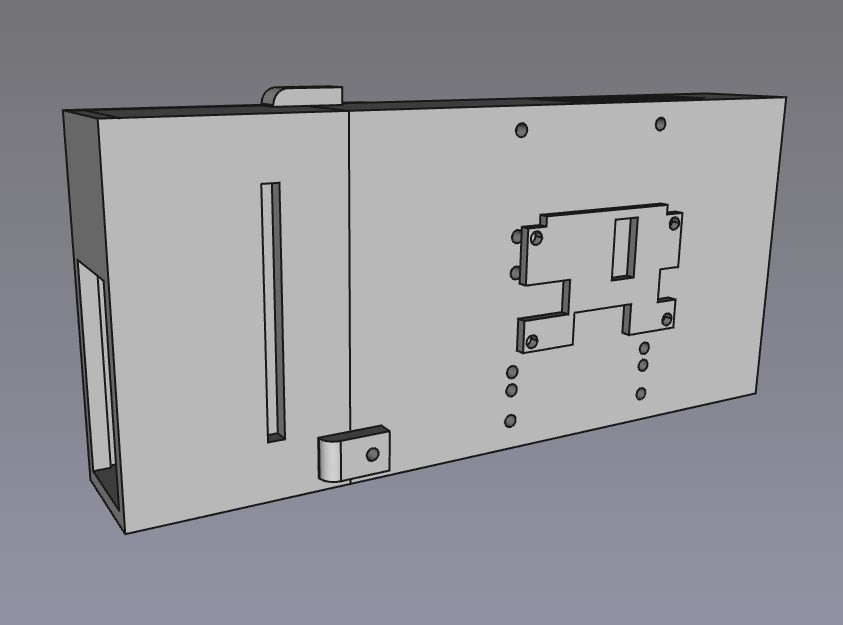
\includegraphics[width=\textwidth]{imgs/freecad/psu_mount.jpg}
      \caption{PSU Housing}
    \end{minipage}
    \hfill
    \begin{minipage}[t]{0.32\textwidth}
      \centering
      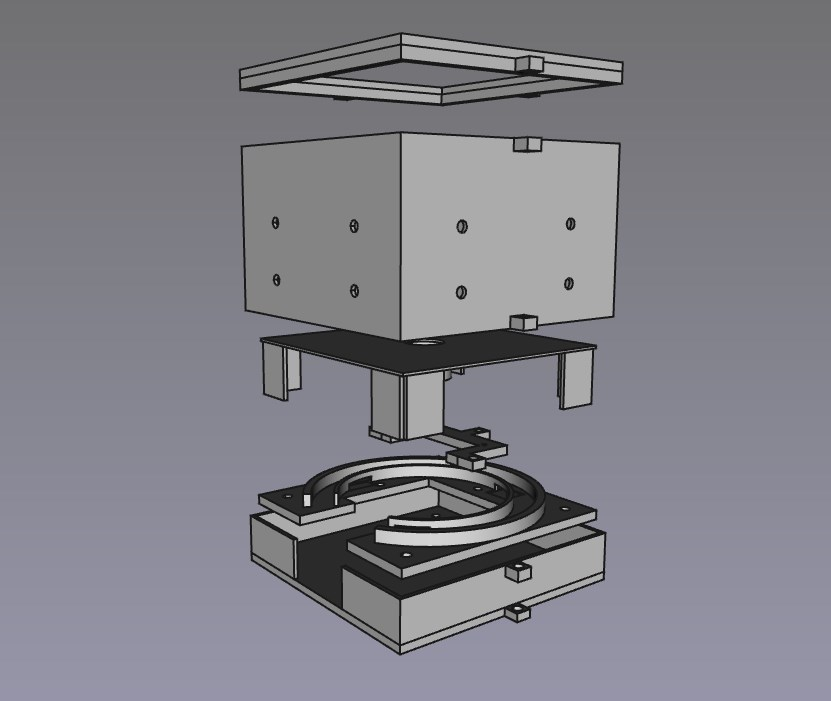
\includegraphics[width=\textwidth]{imgs/freecad/camera_case.jpg}
      \caption{Camera Housing}
      \label{fig:camerahousing}
    \end{minipage}
    \hfill
    \begin{minipage}[t]{0.32\textwidth}
      \centering
      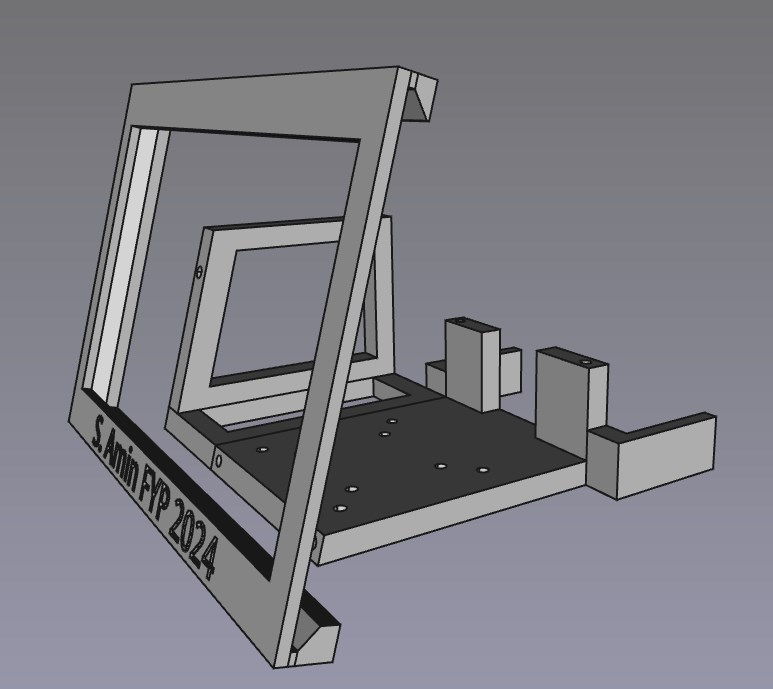
\includegraphics[width=\textwidth]{imgs/freecad/lcd_mount.jpg}
      \caption{LCD Display Housing}
    \end{minipage}
\end{figure*}

% Screen
\vspace{1em}
\noindent
\textbf{7" Touchscreen Display} \\
The DFRobot 7" Touchscreen Display was chosen as it is a relatively cheap display that is compatible with the Raspberry Pi.
It has touchscreen support and has a Raspberry Pi 4 mount on its back, as well as HDMI adapter boards to connect to the Pi.
This means I do not have to design a physical mount for the Pi, and only need to design a mount for the display.

% Power Supply
\vspace{1em}
\noindent
\textbf{24V dc, 6.25A, 150W Power Supply} \\
There are two parameters that were taken into consideration when choosing a power supply: the power output and the voltage.
\begin{mylist}
  \item \textbf{Power Rating} \\
  The power supply must be able to drive all components in the system with overhead in case of spikes in power consumption.
  In this first stage, the system only consists of the Raspberry Pi, the display, LED lights and camera, 
  making for a power consumption of under 20W, recorded using a smart plug with a power meter.
  However, in the future, the system will likely need to drive additional motors and sensors, so the total power consumption
  will be higher. Even with accounting for this, the power consumption will be under 100W, so a 150W power supply will be sufficient,
  allowing a 50W overhead. In hindsight, this may be considered excessive.
  \item \textbf{Voltage Rating} \\
  The voltage of the power supply must be greater or equal than the highest voltage of any component in the system; this is necassary
  as I have only step-down converters available on hand, so choosing a higher voltage allows me to step-down the voltage 
  to the required voltage for each component. 24V was chosen as it is a common voltage for stepper motors, which may be used in
  future stages of the project. It is also used for some LED strips, which are used in this stage. The Pi 4 uses 5V and the LED strip
  uses 12V, which the 24V power supply can be stepped down to.
\end{mylist}

% LED 
\noindent
\textbf{Okdo Adjustable Focus OV5647 Camera} \\
For the Computer Vision system, a camera is required to capture images of the components. The Okdo Adjustable Focus OV5647 Camera
was chosen as it is CSI compatible, meaning it can be connected directly to the Raspberry Pi, and has a manual focus ring, allowing
it to be used as a macro camera to capture images of small components placed directly above it. The manual focus ring allows the camera
to be specifically tuned to the design of the system, allowing for the best possible image quality. It also
has a 5MP sensor\cite{okdospec}, which is sufficient for the Computer Vision system, as high resolution images would be preprocessed and reduced.

% LED
\vspace{1em}
\noindent
\textbf{LED Light Strip} \\
An LED strip is required to illuminate the components so that the camera can capture images of them.
Initially, a 12V LED Ring was chosen as it would allow for a uniform light source and can be mounted directly below the camera; 
however for reasons explained in the next section, it was replaced with a 5V WS2812B LED strip as it solves the issues
faced with the LED Ring.
